\chapter{Implementation}
\label{chap:implementation}

This chapter presents an in-depth description of how \f{} works
and demonstrates how much it can simplify developers' experience
by showing real-world examples with extensive usage of its features.
Furthermore, since we are creating an open-source project, the structure of
the repository will also be analyzed.


\section{Overview}

\f{} is a transpiler which enhances serverless programming by introducing the concept of annotations.
Annotations are an abstraction layer that the developers can unobtrusively use
to apply code transformations and metadata generation to a given application,
which will be deployed to a serverless platform.

To achieve this goal, we used the \textit{TypeScript}\cite{ts} compiler API which lets us
manipulate sources with ease, and \textit{SLS}\cite{sls} which
uses the generated metadata to deploy to \textit{AWS Lambda}.

\begin{figure}[H]
  \centering
  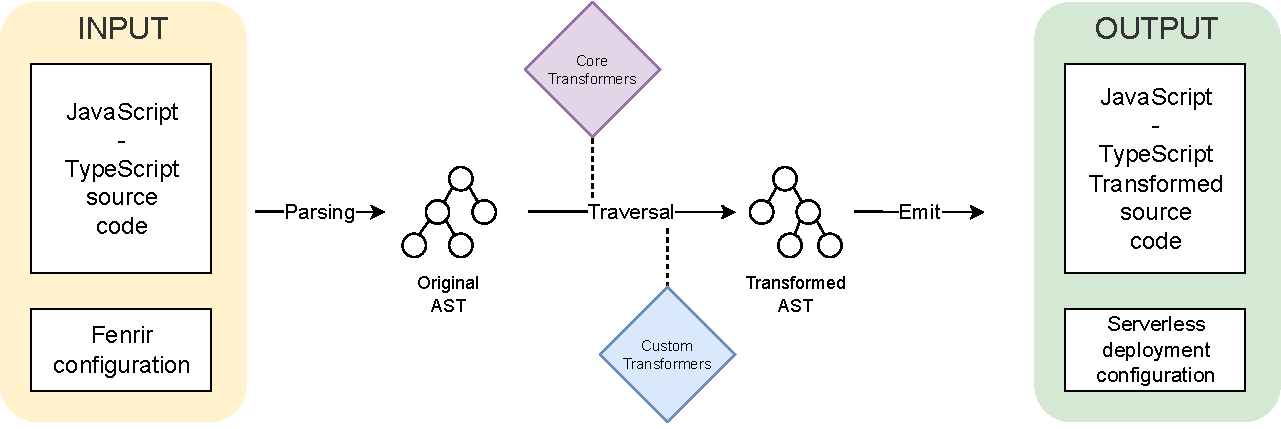
\includegraphics[width=\textwidth]{diagrams/pipeline}
  \caption{Transpiler pipeline.}
  \label{fig:pipeline}
\end{figure}

The transpilation pipeline, depicted in Figure \ref{fig:pipeline},
starts with the parsing of the input source code, which produces AST nodes with their related
annotations. Then, each annotation induces the application of its related
transformation step, whose output is fed into the next transformer, if any.
During the transformation steps, \f{} reports possible errors by gracefully
stopping the compilation process and indicating the offending instructions. Once
the transformations have taken place without any errors, the output code is saved
and the related metadata is also appended to a
\verb|serverless.yml| file which specifies function deployment
properties (e.g., the address to invoke a given function).

It is important to notice that \f{} doesn't lock developers in managing their
functions only through its tools, instead, its primary objective is to facilitate
the incremental adoption of the serverless paradigm.

\subsection{Brief example: Monolith to Serverless conversion}

Lorem ipsum dolor sit amet, qui minim labore adipisicing minim sint cillum sint consectetur cupidatat.

\section{Detailed review}

This section explains each step of the pipeline, defines annotations precisely and shows how to create new ones.

\subsection{Parsing}

\f{} requires a configuration file, that must be named \verb|fenrir.config.json|, to understand where to operate:

\begin{lstlisting}[language=json]
{
  "files": ["input/source.ts"],
  "serverlessConfigPath": "input/serverless.yml",
  "outputDirectory": "output",
  "annotations": {
    "CustomAnnotation": "annotations/custom-annotation.ts"
  }
}
\end{lstlisting}

The \verb|files| field accepts an array of filenames or an entire directory,
and it is used to represent which files will be parsed by the transpiler.

The \verb|serverlessConfigPath| field points at the input \textit{SLS} configuration
that must contain some mandatory input metadata, such as the region which the functions will be deployed on.

The \verb|outputDirectory| field indicates where the emitted files will be placed.

The \verb|annotations| field locates custom annotations as it takes an object
where the keys represent the new names and the values refer to their associated implementations.

\paragraph{\textbf{Fenrir's CLI}}
After creating the configuration, \f{} can be started through our CLI tool
by optionally passing as a flag the directory in which it is contained.
\begin{lstlisting}[language=bash, style=bashstyle]
# defaults to the current directory (.) for its file lookup...
> fenrir
# ...or uses a custom path
> fenrir -g input-directory
\end{lstlisting}

\subsection{Core annotations}

Lorem ipsum dolor sit amet, qui minim labore adipisicing minim sint cillum sint consectetur cupidatat.

\subsection{Emit}

Magari parlare della gestione degli errori. E poi dell'emit.
